\section{Background and Related Work}

Figure~\ref{technology} illustrates the fundamentals of the most promising emerging memory technologies to be investigated in our project, namely, the Phase-Change RAM (PCRAM), the Magnetic RAM (MRAM) based on Spin-Torque Transfer RAM(STT-RAM), the resistive RAM (RRAM), and the memristor. In this section, we will briefly describe the physical mechanisms of the emerging NVM devices. The research and development related to this proposal will also be described.

\subsection{Phase-Change RAM (PCRAM)}
PCRAM technology is based on a chalcogenide alloy (typically, Ge$_2$--Sb$_2$--Te$_5$, GST) material, which is similar to those commonly used in optical storage means (compact discs and digital versatile discs)~\cite{Bedeschi09}. The data storage capability is achieved from the resistance differences between an amorphous (high-resistance) and a crystalline (low-resistance) phase of the chalcogenide-based material as shown in Figure~\ref{technology}. In SET operation, the phase change material is crystallized by applying an electrical pulse that heats a significant portion of the cell above its crystallization temperature. In RESET operation, a larger electrical current is applied and then abruptly cut off in order to melt and then quench the material, leaving it in the amorphous state~\cite{burr:scm08}. 

PCRAM has shown to offer compatible integration with CMOS technology~\cite{Oh06}, fast speed~\cite{Pirovano03}, high endurance~\cite{Lai03}, and inherent scaling of the phase-change process at 22-nm technology node and beyond~\cite{Chen06}. Compared to STT-RAM, PCRAM is even denser with an approximate cell area of $6\sim12F^2$~\cite{ITRS07}, where F is the feature size. In addition, phase change material has a key advantage of the excellent scalability within current CMOS fabrication methodology~\cite{Cho05,Kim06,Lai01,Pirovano03,Raoux08}, with continuous density improvement~\cite{Nirschl07,Chen07-iedm,Im08}. 

Although many device models were built from reliability~\cite{Ielmini07}, low-frequency noise~\cite{Fantini08}, statistical analysis~\cite{Mantegazza07} point of views, they were mainly dedicated to process and device, which cannot be directly borrowed by circuit design and computer community. Many PCRAM prototypes have been demonstrated in the past years by companies like Hitachi~\cite{Hanzawa07}, Samsung~\cite{Lee07-isscc}, STMicroelectronics~\cite{Bedeschi08, Sandre10}, and Numonyx~\cite{Villa10}. The maximum capacities achieved are 1Gb and 256Mb for single level cell (SLC)~\cite{Villa10} and multi-level cell (MLC)~\cite{Lee07-isscc}, respectively. However, to be more competitive to the existing DRAM and Flash memory, PCM need further improvement on density and endurance. In this project, we will address this issue mainly from circuit design point of view. 

\begin{figure}
\centering
%\vspace{-10pt} 
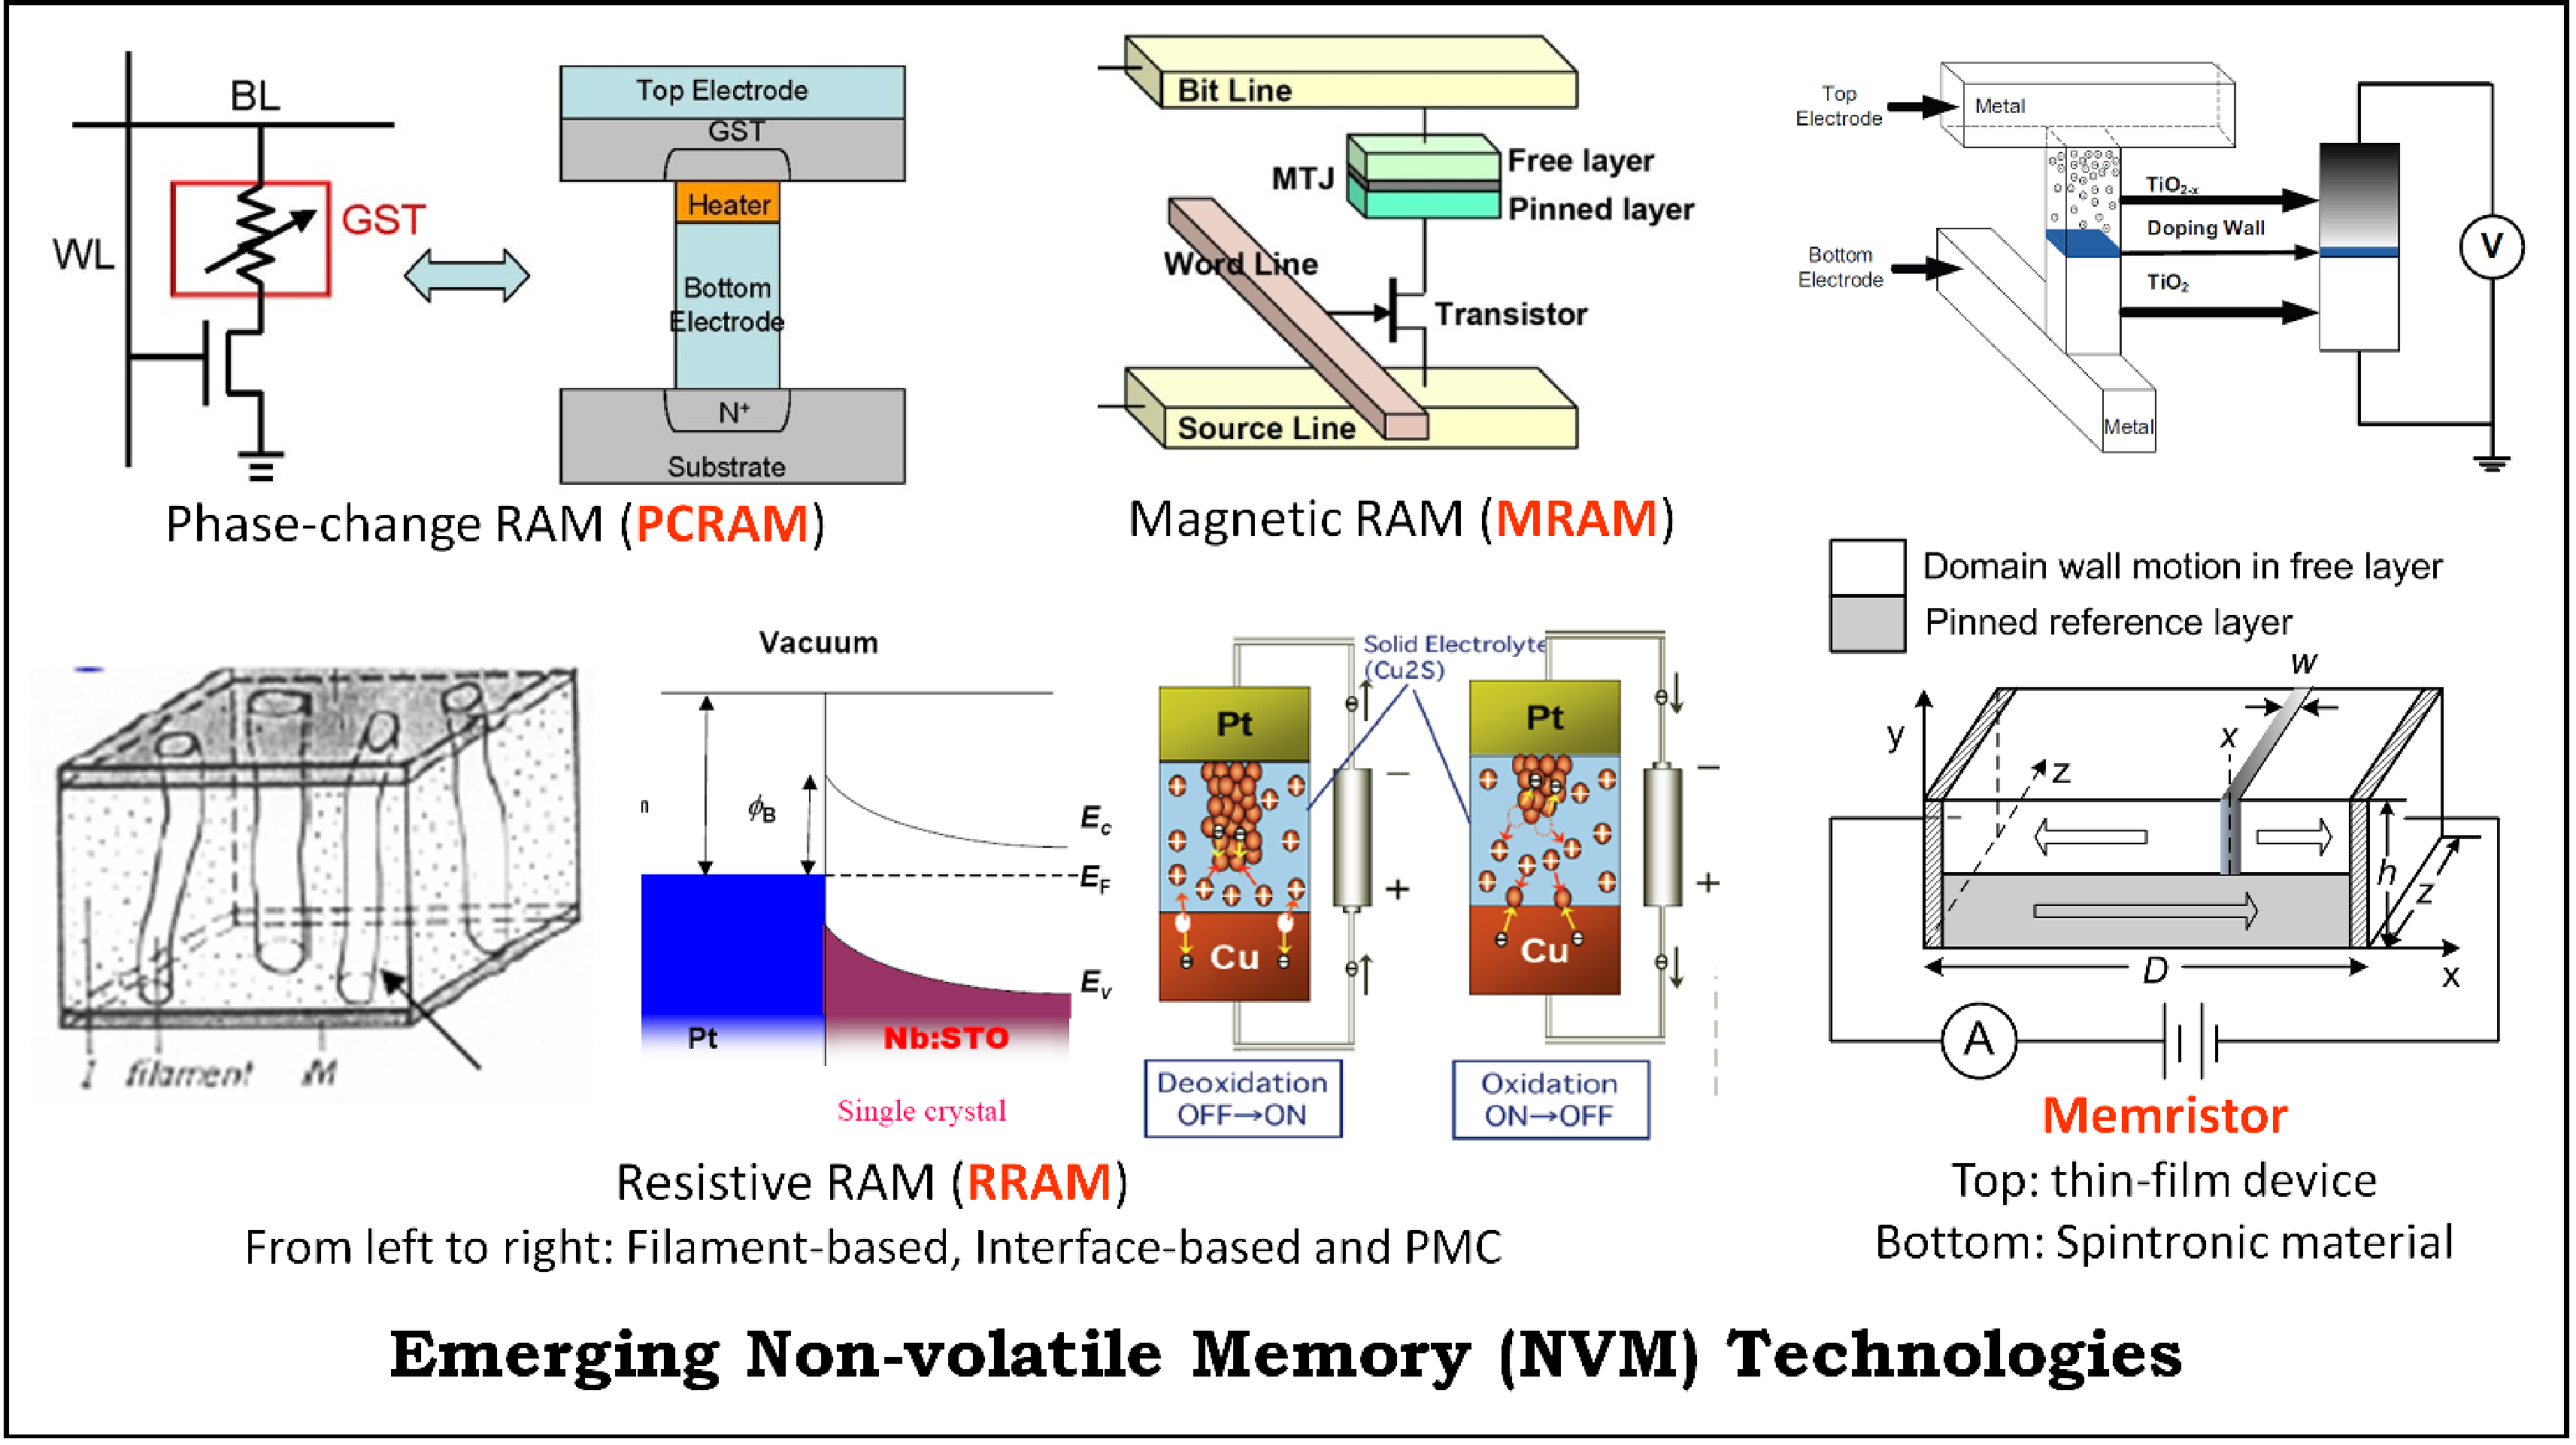
\includegraphics[width=0.9\textwidth]{./figure/1_technology_half.pdf} 
\vspace{-10pt}
\caption{\textbf{Overview of Some Emerging Non-volatile Memory Technologies} including Phase-Change RAM (PCRAM), Magnetic RAM (MRAM), resistive RAM (RRAM), and memristor. }
\label{technology} 
\vspace{-10pt}
\end{figure}

\subsection{MRAM based on Spin-Torque Transfer RAM (STT-RAM)}
STT-RAM is a new type of Magnetic RAM (MRAM)~\cite{ITRS07,Hosomi05,MRAM:TTO+06,MRAM:ZBM+06,mram:ibm:maffitt}, which features non-volatility, fast writing/reading speed (\textless 10ns), high programming endurance (\textgreater 10$^{15}$cycles) and zero standby power~\cite{ITRS07}. The storage capability or programmability of MRAM arises from magnetic tunneling junction (MTJ), in which a thin tunneling dielectric, e.g., MgO., is sandwiched by two ferromagnetic layers, as shown in Figure~\ref{technology}. One ferromagnetic layer (``pinned layer'') is designed to have its magnetization pinned, while the magnetization of the other layer (``free layer'') can be flipped by a write event. An MTJ has a low (high) resistance if the magnetizations of the free layer and the pinned layer are parallel (anti-parallel). In first-generation MRAM design, the magnetization of free layer is changed by the current-induced magnetic field~\cite{Motoyoshi04,Ha04}. In STT-RAM, a new write mechanism called ``polarization-current-induced magnetization switching'' is introduced -- the magnetization of free layer is flipped by the electrical current directly. Because the current required to switch an MTJ resistance state is proportional to the MTJ cell area, STT-RAM is believed to have a better scaling property than the first-generation MRAM~\cite{Hosomi05,Kawahara07,MRAM:TTO+06,Diao07,Salahuddin07,Beach08,Kishi08}.

Continuous efforts on process development have been taken on yield improvement~\cite{Miura07}, write power reduction~\cite{Durlam03}, and high density~\cite{Lou08}.

Prototyping STT-RAM chips have been demonstrated recently by various companies and research groups~\cite{Hosomi05,Kawahara07,Nebashi09,Motoyoshi04,Andre05,Kawahara08}. Commercial MRAM products have been launched by companies like Everspin (which is a spin-off from Freescale to expedite the technology commercialization in 2008) and NEC.




A 4Kb STT-RAM using tailored MTJ design was fabricated by Sony in $0.18{\mu}m$ technology in 2005~\cite{Hosomi05}. The test chip demonstrated that STT-RAM is a prominent candidate for the next generation memory because of its high speed, low power and high scalability. In 2007, Kawahara et al. prototyped a larger 2Mb STT-RAM in $0.2{\mu}m$ technology~\cite{Kawahara07}. This chip improves memory access latency by featuring an array scheme with bit-by-bit bidirectional current write and a parallelizing-direction current read. Recently, a even larger capacity -- 32Mb MRAM prototype in 90nm technology was demonstrated by NEC~\cite{Nebashi09}. A cell structure with 2 transistors and 1 magnetic tunneling junction (2T1MTJ) was adopted to improve access time to 12ns. Besides the SRAM-like array~\cite{Motoyoshi04,Andre05,Kawahara08}, other memory structures are also investigated by using MRAM/STT-RAM technology. In~\cite{Wang07}, Wang et. al. described a CAM structure based on conventional MRAM technology. In~\cite{Xu08}, Wu et. al. propsoed a novel STT-RAM read scheme with high sensing margin and illustrates a new CAM design. The possibility of applying STT-RAM in reconfigurable logic block for 3D-stacked reconfigurable spin processor was investigated~\cite{Sekikawa08}.

A write disturbance fault (WDF) model for conventional MRAM was proposed by Su et al.~\cite{Su08}. The fault affects the data stored in MRAM cells due to excessive magnetic filed during a write operation.
This should not be a problem to STT-RAM since it uses spin-polarized current to flip data. We have proposed a dynamic MTJ model with more accurate (transient) description for MTJ resistance switching~\cite{Chen08}. Compared to highly conceptual fixed resistance used in traditional STT-RAM design flow, the dynamic model can help to reduce 20\% pessimism in write time at TSMC $0.13{\mu}m$. The failure probability of STT-RAM cells due to parameter variations was considered and discussed in~\cite{Li09}. A model was proposed to predict memory yield and design optimization to minimize memory failures.





\subsection{Resistive RAM (RRAM)}
RRAM can generally denote all the memory technologies that rely on the resistance change to store the data. Based on the storage mechanisms, RRAM materials can be cataloged as space-charge-limited-current (SCLC), filament, programmable-metallization-cell (PMC), Schottky contact and traps (SCT), etc.

Among them, filament-based RRAM, a typical example of unipolar switching~\cite{Inoue}, has been widely investigated because of the potentials on high-speed, high-endurance, and better scalability. The insulating material between two electrodes can be made conducting through a hopping or tunneling conduction path after the application of a sufficiently high voltage, a process called electro-forming. The data storage could be achieved by break (RESET) or reconnect (SET) the conducting path. Such switching mechanism can in fact be explained with the fourth circuit element, i.e., the memristor or the memory resistor~\cite{Chua71,Tour08,Strukov08}. Indeed, HP Labs plan to unveil RRAM prototype chips based on memristor with crossbar arrays soon.

PMC~\cite{Kozicki05} is a promising bipolar switching technology, which is composed of two solid metal electrodes -- relatively, one is inert and the other is electrochemically active. Between the two electrodes locates a thin electrolyte film. When a negative bias is applied to the inert electrode in programming operation, metal ions in the electrolyte together with those flew from the positive active electrode can be reduced by the inert electrode. As a result, the metal ions form a small metallic ``nanowire'' between the two electrodes, which produces a low resistance. In erasing operation, a positive bias is applied on the inert electrode. metal ions migrate back into the electrolyte and eventually to the negatively-charged active electrode. The ``nanowire'' is broken and the resistance increase back.

\subsection{Memristor}
Memristor, the fourth fundamental passive circuit element, was predicted by Professor Chua in 1971~\cite{Chua71}, based on the completeness of circuit theory. Different from other electrical parameters resistance (\textit{R}), capacitance (\textit{C}) and inductance (\textit{L}), memristance (\textit{M}) is a function of charge (\textit{q}),  which depends upon the historic behavior of the current (or voltage) profile~\cite{Chua76}. In 2008, 37 years after memristor was predicted in theory, the researchers at HP reported the first real device of a memristor. The memristive effect was achieved in a solid-state thin film two-terminal device by moving the doping front along the device~\cite{Tour08}. Afterwards, magnetic technology provides the other possible methods to build a memristive system~\cite{Pershin08,Wang09}. Due to its unique historic characteristic, memristor has very broad application including nonvolatile memory, signal processing, control and learning system etc~\cite{Chen09}.


\begin{figure}
%\begin{wrapfigure}{r}{0.6\textwidth}\centering
\centering
\vspace{-10pt} 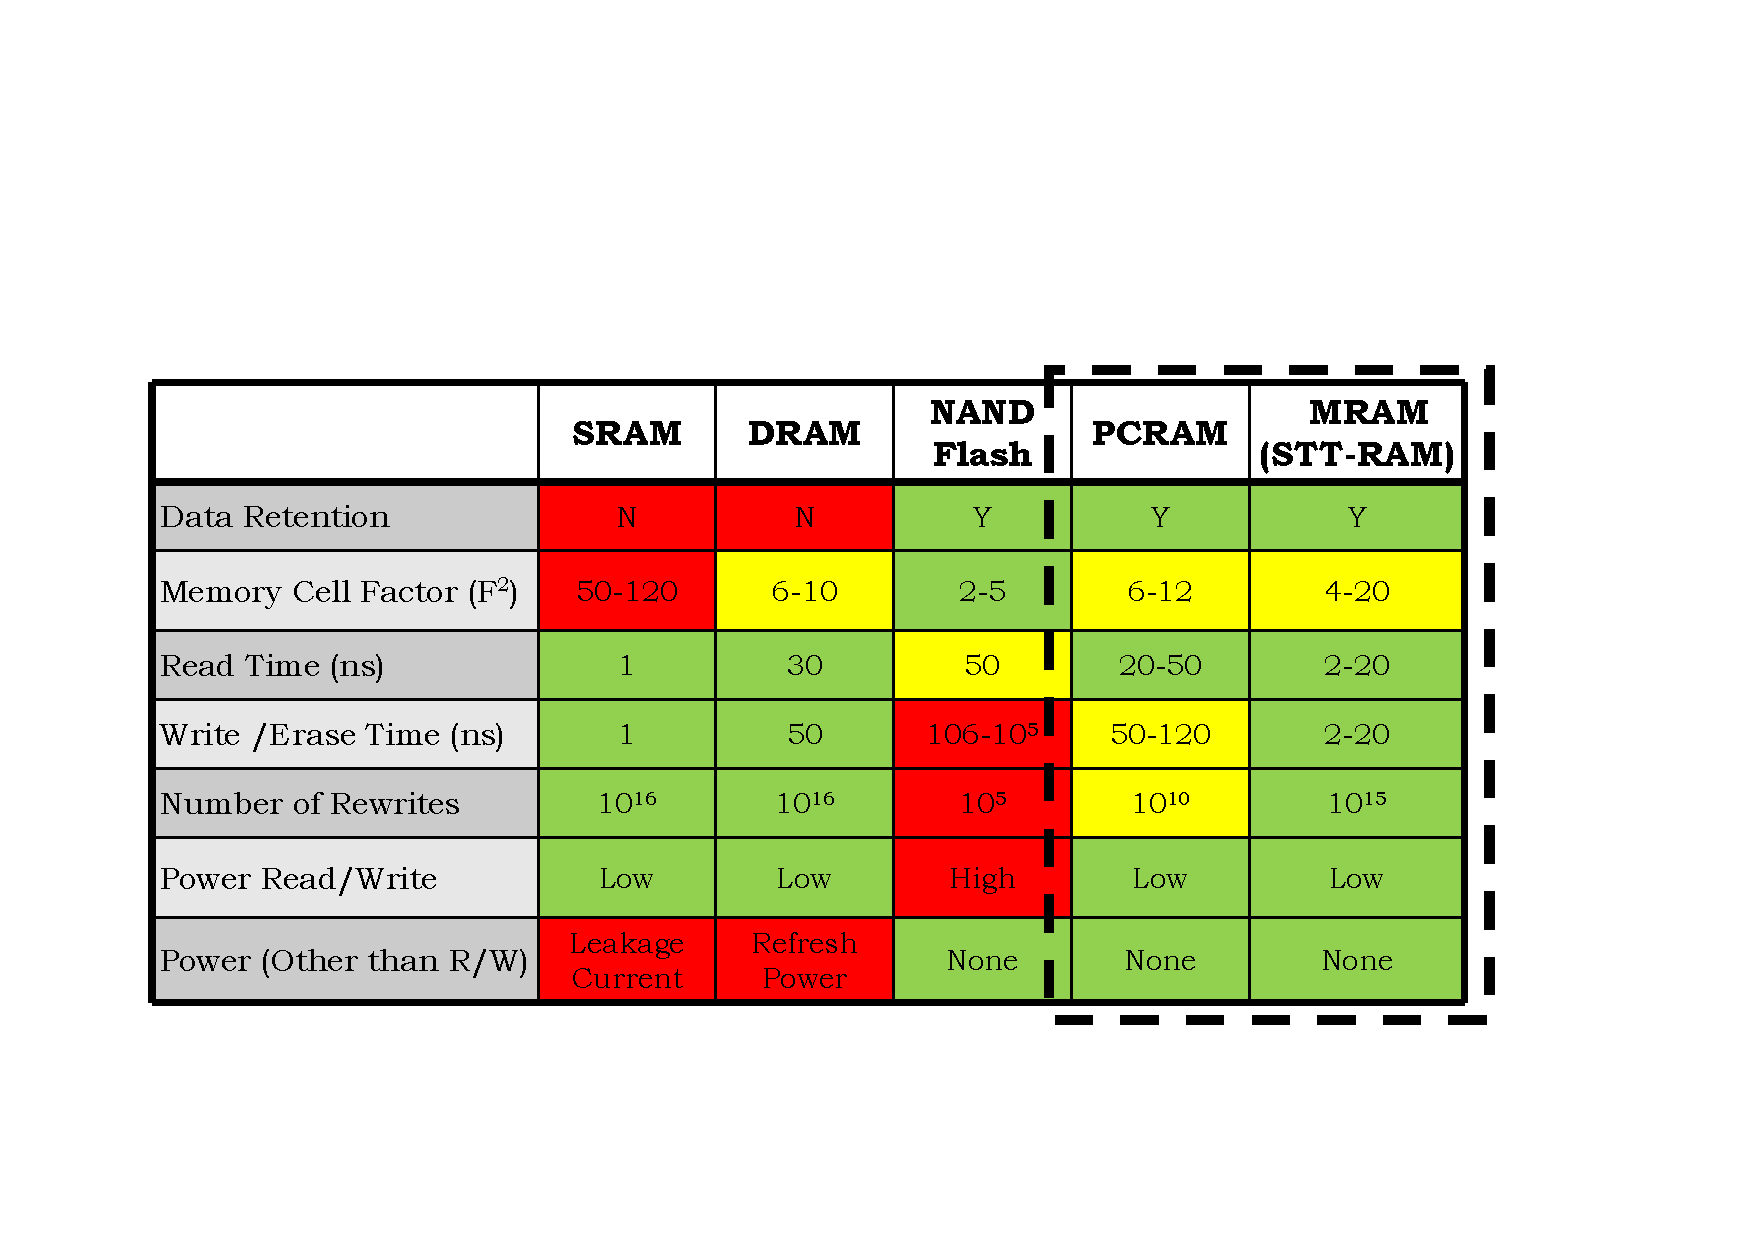
\includegraphics[width=0.7\textwidth]{./figure/table.pdf} \vspace{-10pt}
\caption{The comparison of various memory
technologies~\cite{ITRS07}.}\label{table} \vspace{-10pt}
%\end{wrapfigure}
\end{figure}

\paragraph{Summary}
Figure~\ref{table} illustrates the comparison of
two emerging memory technologies -- PCRAM and MRAM (STT-RAM)  --
against the traditional main-stream SRAM, DRAM, and NAND-based Flash memory~\cite{ITRS07}.
Note that both CMOS-compatible embedded MRAM (NEC)~\cite{MRAM:NEC09} and embedded PCRAM (Hitachi and STMicro)~\cite{PRAM:Hitachi2007,PRAM:ST2004} have been demonstrated, paving the way of integrating
these NVMs to the traditional memory hierarchies. In addition, the emerging 3D integration technologies~\cite{xie:jetcs06,Xie:dac08}
enables cost-effective integration of these NVMs with CMOS logic circuits. With all the NVM technology advances in recent years, it is anticipated that the emerging NVM technologies will break important ground and move closer to market in the near future (``Non-volatile memory goes commercial", EEtimes, 12/02/2009).


